\definecolor{Planung}{HTML}{FF1111}
\definecolor{Backend}{HTML}{00FFC1}
\definecolor{ACP}{HTML}{2F95DE}
\definecolor{Seite}{HTML}{299819}
\definecolor{Dokumentation}{HTML}{2300E7}

\definecolor{Technologie}{HTML}{4F81BD}
\definecolor{PlanungApp}{HTML}{C0504D}
\definecolor{App}{HTML}{9BBB59}
\definecolor{Funktionalitaet}{HTML}{8064A2}
\definecolor{DokumentationApp}{HTML}{4BACC6}

\section*{Arbeitsprotokoll - Philipp Schuler}

\begin{table}[H]
    \begin{tabular}{lrr}
        \hline
        \textbf{Projektteil}  & \textbf{Arbeitsaufwand} & \textbf{Prozentueller Anteil} \\ \hline
        \fcolorbox{black}{Technologie}{\rule{0pt}{4pt}\rule{4pt}{0pt}} Technologie erlernen & 32:57:00                & 17,16\%                       \\
        \fcolorbox{black}{PlanungApp}{\rule{0pt}{4pt}\rule{4pt}{0pt}} Planung               & 7:31:12                 & 3,92\%                        \\
        \fcolorbox{black}{App}{\rule{0pt}{4pt}\rule{4pt}{0pt}} App Design und Aufbau        & 48:35:25                & 25,30\%                       \\
        \fcolorbox{black}{Funktionalitaet}{\rule{0pt}{4pt}\rule{4pt}{0pt}} Funktionalität   & 75:25:09                & 39,27\%                       \\
        \fcolorbox{black}{DokumentationApp}{\rule{0pt}{4pt}\rule{4pt}{0pt}} Dokumentation   & 27:34:50                & 14,36\%                       \\ \hline
        \textbf{Summe}        & \textbf{192:03:36}      & \textbf{100,00\%}             \\ \hline
    \end{tabular}
\end{table}

\begin{figure}[H]
    \begin{center}
        \includegraphics[width=0.8\textwidth]{Appendix/Philipp/Kuchen.png}
        \caption{Verteilung von Philipps Arbeitsstunden}
    \end{center}
\end{figure}

\begin{figure}[H]
    \begin{center}
        \includegraphics[width=1\textwidth]{Appendix/Philipp/Balken.png}
        \caption{Philipps Arbeitsverlauf vom 30.11.2021 bis zum 24.03.2022}
    \end{center}
\end{figure}

\newpage

\section*{Arbeitsprotokoll - Alexander Bertoni}

\begin{table}[H]
    \begin{tabular}{lrr}
        \hline
        \textbf{Projekt}                                                               & \multicolumn{1}{l}{\textbf{Arbeitsaufwand}} & \multicolumn{1}{l}{\textbf{Prozent}} \\ \hline
        \fcolorbox{black}{Planung}{\rule{0pt}{4pt}\rule{4pt}{0pt}} Planung             & 2:41:10                                     & 1.40\%                               \\
        \fcolorbox{black}{Seite}{\rule{0pt}{4pt}\rule{4pt}{0pt}} Seite                 & 153:25:45                                   & 79.78\%                              \\
        \fcolorbox{black}{Dokumentation}{\rule{0pt}{4pt}\rule{4pt}{0pt}} Dokumentation & 36:12:34                                    & 18.82\%                              \\
        \hline
        \textbf{Summe}                                                                 & \textbf{192:19:29}                          & \textbf{100.00\%}                    \\
        \hline
    \end{tabular}
\end{table}

\begin{figure}[H]
    \begin{center}
        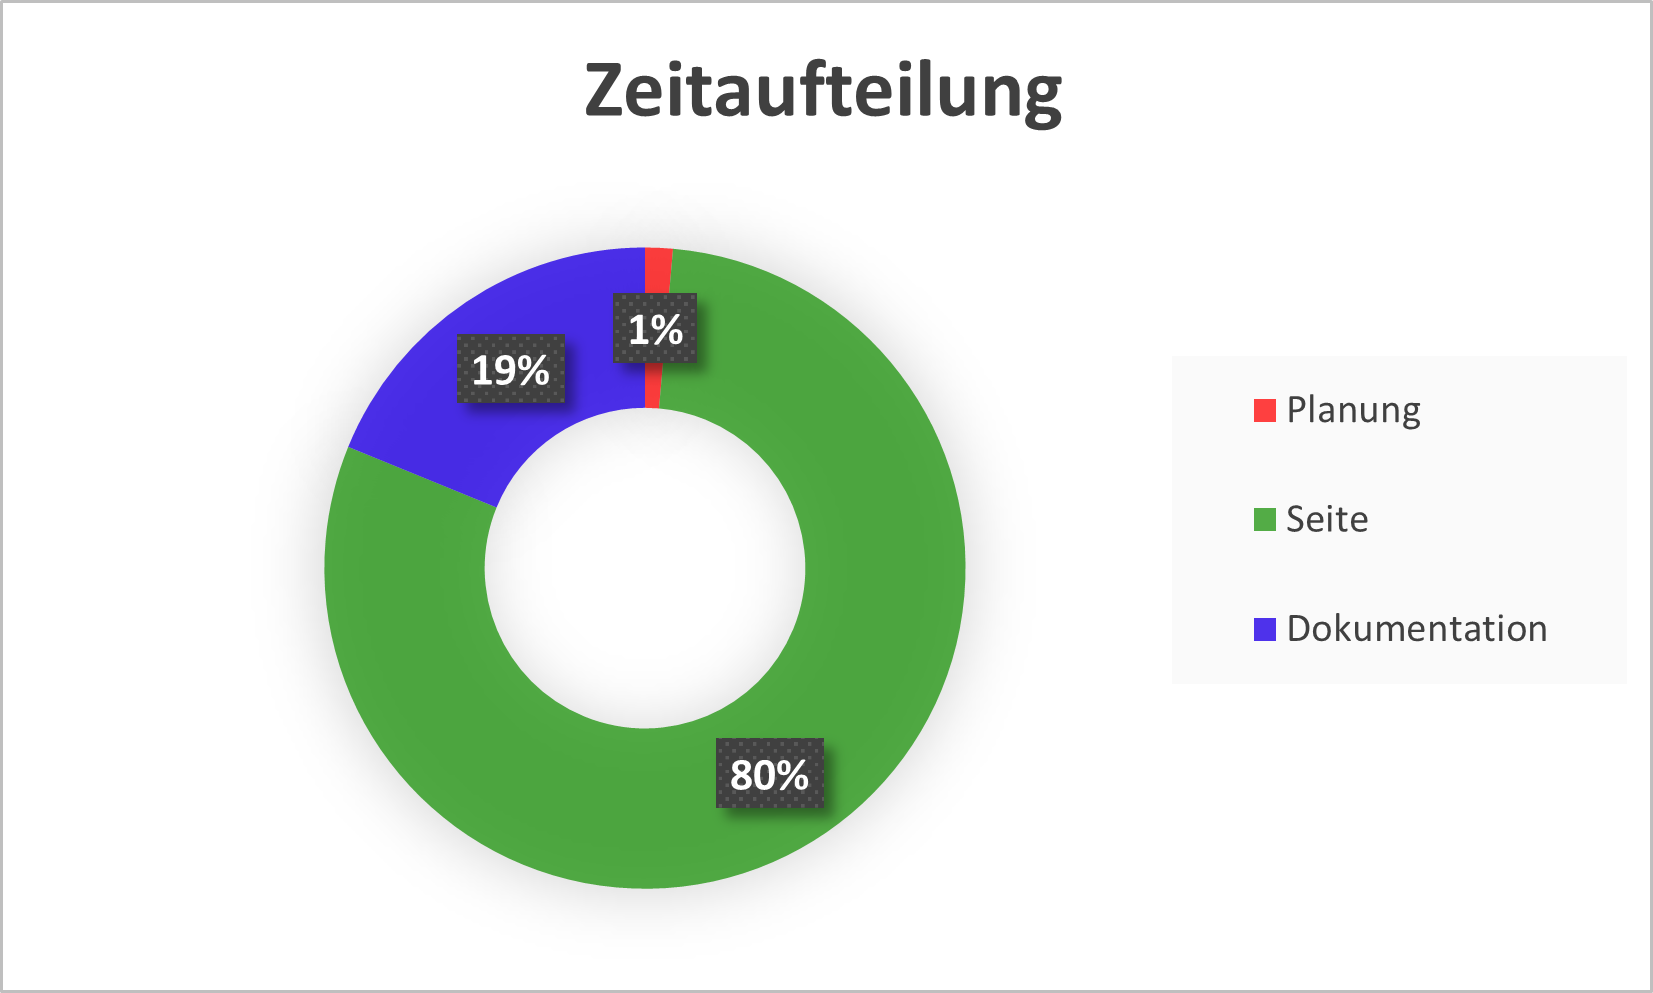
\includegraphics[width=1\textwidth]{images/Zeiten/Zeitaufteilung-Bertoni.png}
        \caption{Verteilung von Alexanders Arbeitsstunden}
    \end{center}
\end{figure}

\begin{figure}[H]
    \begin{center}
        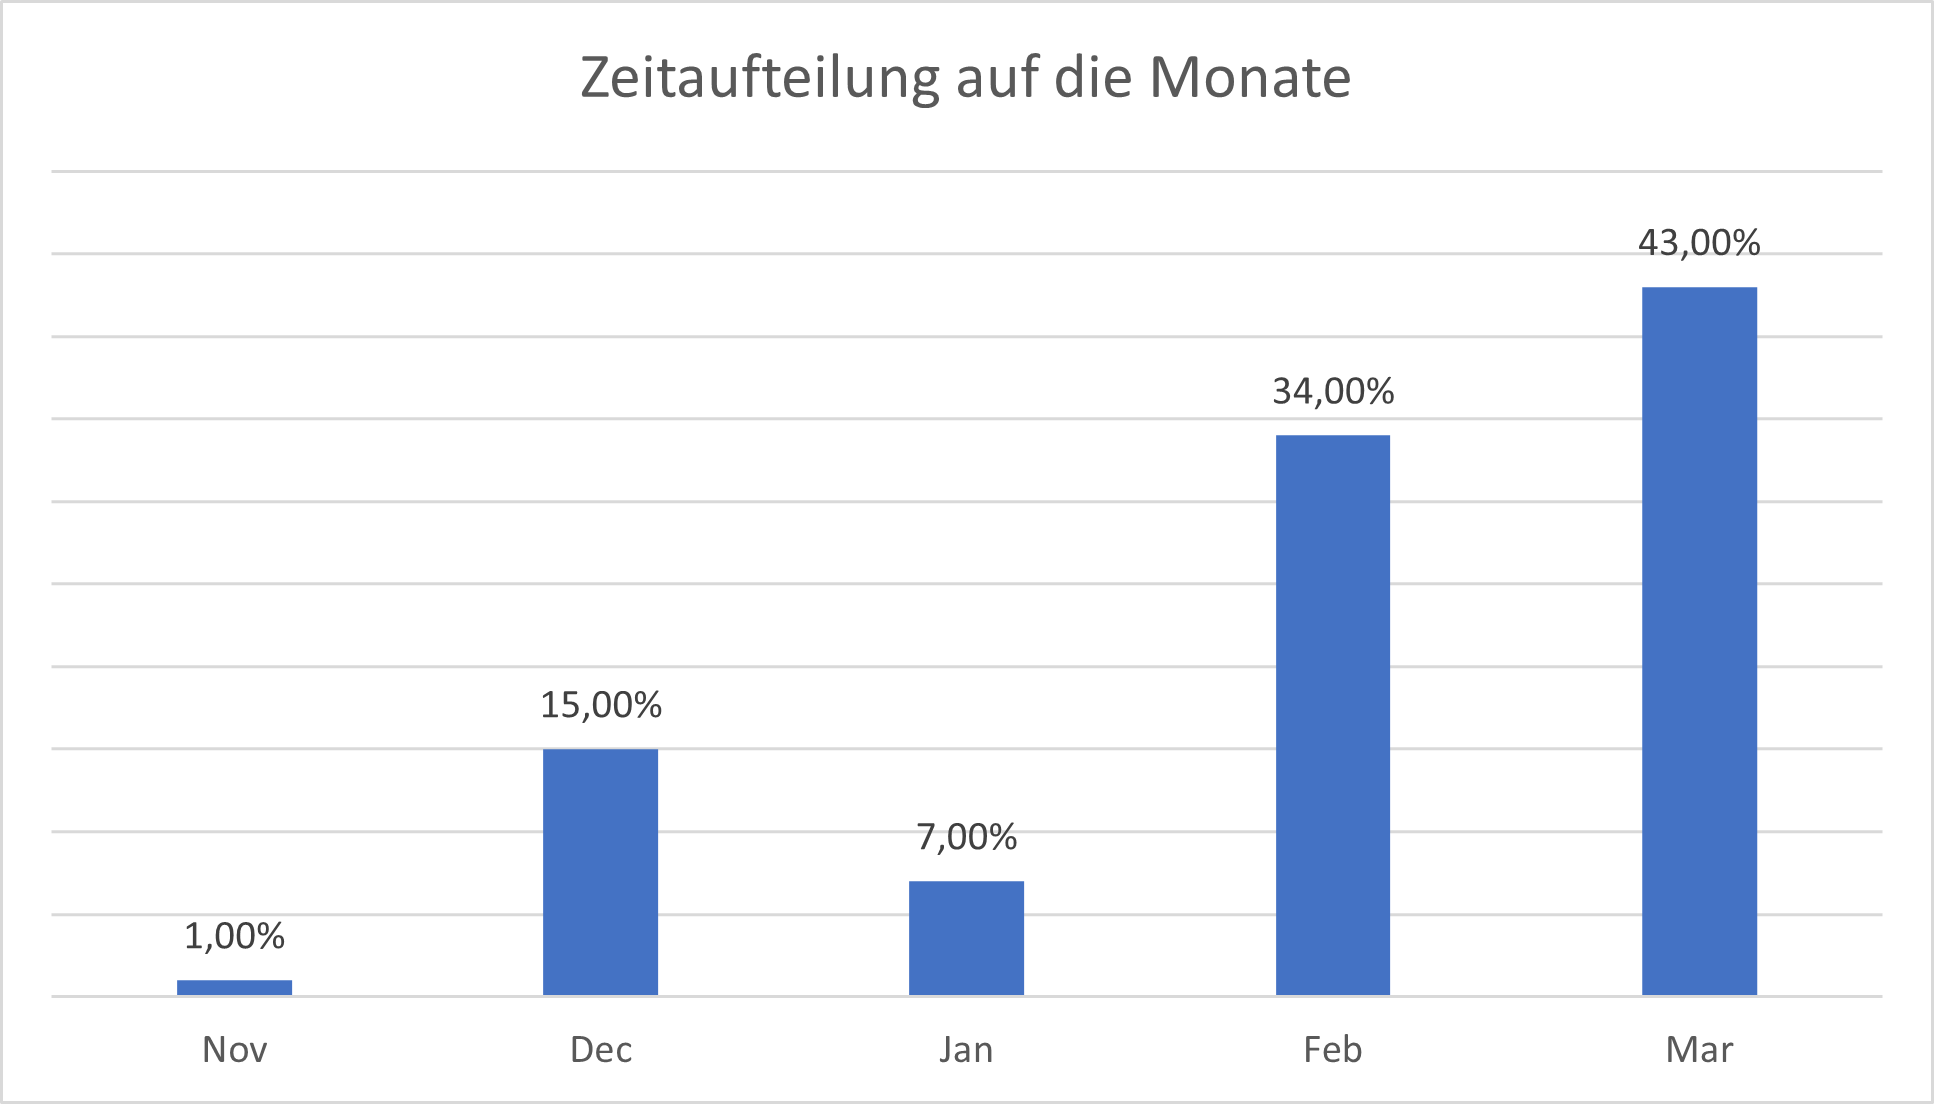
\includegraphics[width=1\textwidth]{images/Zeiten/Zeitaufteilung-auf-Monate-Bertoni.png}
        \caption{Alexanders Arbeitszeiten vom 07.12.2021 bis zum 24.03.2022}
    \end{center}
\end{figure}

\newpage

\section*{Arbeitsprotokoll - Maximilian Neuner}

\begin{table}[H]
    \begin{tabular}{lrr}
        \hline
        \textbf{Projektteil} & \textbf{Arbeitsaufwand} & \textbf{Prozentueller Anteil} \\ \hline
        Technologie erlernen & 28:40:12                & 15,73\%                       \\
        Planung              & 8:31:12                 & 4,49\%                        \\
        Backend Entwicklung  & 103:31:25               & 57,86\%                       \\
        Dokumentation        & 37:35:50                & 20,78\%                       \\ \hline
        \textbf{Summe}       & \textbf{178:34:39}      & \textbf{100,00\%}             \\ \hline
    \end{tabular}
\end{table}

\begin{figure}[H]
    \begin{center}
        \includegraphics[width=1\textwidth]{Appendix/Maximilian/Kuchen.png}
        \caption{Verteilung von Maximilians Arbeitsstunden}
    \end{center}
\end{figure}

\begin{figure}[H]
    \begin{center}
        \includegraphics[width=1\textwidth]{Appendix/Maximilian/Balken.png}
        \caption{Maximilians Arbeitsverlauf vom 30.11.2021 bis zum 24.03.2022}
    \end{center}
\end{figure}
